\documentclass[journal]{IEEEtran}
\usepackage[a5paper, margin=10mm, onecolumn]{geometry}
\usepackage{tfrupee}
\usepackage{amsmath, amssymb, amsfonts, amsthm}
\usepackage{algorithmic}
\usepackage{graphicx}
\usepackage{textcomp}
\usepackage{xcolor}
\usepackage{txfonts}
\usepackage{listings}
\usepackage{enumitem}
\usepackage{mathtools}
\usepackage{gensymb}
\usepackage{comment}
\usepackage[breaklinks=true]{hyperref}
\usepackage{tkz-euclide} 
\usepackage{listings}
\usepackage[latin1]{inputenc}                                
\usepackage{color}                                            
\usepackage{array}                                            
\usepackage{longtable}                                       
\usepackage{calc}                                             
\usepackage{multirow}                                         
\usepackage{hhline}                                           
\usepackage{ifthen}                                           
\usepackage{lscape}
\newcommand{\myvec}[1]{\begin{pmatrix} #1 \end{pmatrix}}

\begin{document}

\bibliographystyle{IEEEtran}
\vspace{3cm}

\title{NCERT-9.7.2.3}
\author{EE24BTECH11042 - SRUJANA}
{\let\newpage\relax\maketitle}

\renewcommand{\thefigure}{\theenumi}
\renewcommand{\thetable}{\theenumi}
\setlength{\intextsep}{10pt} 

\numberwithin{equation}{enumi}
\numberwithin{figure}{enumi}
\renewcommand{\thetable}{\theenumi}

\textbf{QUESTION}:\\

Verify that the given function is a solution of the corresponding differential equation.\\

$\frac{d^2y}{dx^2}+9y-6cos3x = 0  :  y = xsin3x\\$

\textbf{Theoretical Solution:\\}

\begin{align}
   \frac{d^2y}{dx^2} &= 6 \cos{3x} -9y 
\end{align}

Solution have two parts homogeneous solution and particular solution

\textbf{Homogeneous part :}
\begin{align}
    \frac{d^2y}{dx^2} = -9y
\end{align}

assume solution is of the form $ce^{rx}$

\begin{align}
    r^2 &= -9\\
    r &= \pm 3i
\end{align}

As the roots are exponential  , then the solution will be of the form $C_1cos3x + C_2sin3x$

\textbf{Particular solution:}\\

Since the non-homogeneous term is \( 6 \cos 3x \), which is a trigonometric function, we assume the particular solution has the same form:
\begin{align}
   y_p(x) = A x \cos 3x + B x \sin 3x
\end{align}

First derivative:
\begin{align}
    y_p'(x) &= A \cos 3x - 3Ax \sin 3x + B \sin 3x + 3Bx \cos 3x 
\end{align}

Second derivative:
\begin{align}
    y_p''(x) = -6A \sin 3x -6Ax \cos 3x + 6B \cos 3x - 6Bx \sin 3x 
\end{align}

Now substitute \( y_p(x) \) and \( y_p''(x) \) into the original differential equation \( \frac{d^2y}{dx^2} = 6 \cos 3x  \) - 9y.\\

Simplifying and comparing coefficients gives the values of \( A \) and \( B \).

we get A = 0 and B =1 \\

Assume  Initial Conditions as 0,0\\

Overall solution $y_h+y_p=y$
 \begin{align}
     y(0) &= C_1 = 0\\
     y''(x) &= 6 \cos{3x} + C_2 \cos 3x\\
     y''(0) &= 6 + C_2
 \end{align}
 
 But , 
 \begin{align}
     y''(0) &= 6 \\
     C_2 = 0
 \end{align}

 Final solution is $y = x \sin{3x}$\\

\textbf{Programming appproach }\\

\textbf{Step 1 : \\}

Using Taylor's expansion around a point \( x \), we approximate \( y(x+h) \) as:\\
\begin{align}
y(x+h) \approx y(x) + h y'(x) + \frac{h^2}{2} y''(x)
\end{align}

we can neglect $y'(x)$ as its contribution to the solution is minimal.\\
\begin{align}
y(x+h) \approx y(x) + \frac{h^2}{2} y''(x),
\end{align}

By substituting x as 0 , $y''(x)$ as 6 and h as 0.01 we get y(h)

\textbf{Step II :}\\

\textbf{Finite differences method}\\

The finite difference method is used to calculate the solutions of differential equations.\\

\begin{align}
    \frac{dy}{dx} &= \lim_{h \to 0}\frac{f(x+h)-f(x)}{h}
\end{align}

Similarly ,
\begin{align}
    y''(x) \approx \frac{y(x+h) + y(x-h) - 2y(x)}{h^2}.
\end{align}
\begin{align}
     y_{n+1} &= \frac{d^2y}{dx^2} \cdot h^2 - y_{n-1} + 2y_{n}\\
     y_{n+1} &= (6 \cos 3x_{n} - 9y_{n}n) \cdot h^2 - y_{n-1} + 2y_{n}\\
    x_{n+1} &= x_{n} + h
\end{align}

By substituting the results obtained above, we calculate $y(-h)$ , \\

Now, use $x+h$ and $f(x+h)$ as the new initial conditions.\\ 

Repeat this process until you have sufficient points to plot the graph. \\

Connect all points to obtain an approximate plot of the differential equation. \\

This is a graphical representation of both the simulation and theoretical approaches of the differential equation.

\begin{figure}[h!]
   \centering
   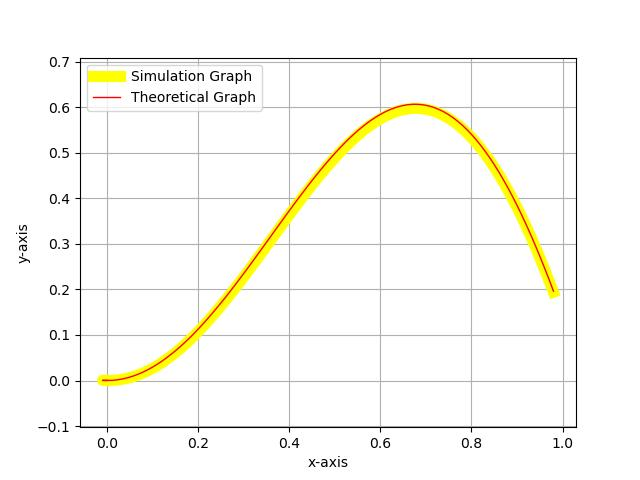
\includegraphics[width=\columnwidth]{fig/combined_fig.jpg}
\end{figure}


\end{document}

